\chapter{Trabalhos Correlatos}

As próximas seções apresentam os mais recentes trabalhos com temática ou abordagem semelhante.

\section{Visão Geral}

Durante a pesquisa por bibliografia que trata especificamente do problema da identificação de documentos falsificados, foram encontrados poucos resultados, sobretudo no âmbito acadêmico, já que a maioria dos trabalhos com temática similar aborda a classificação de fraudes -- dificuldade ilustrada pela tabela \ref{tab:bibliography}, que apresenta a bibliografia obtida que trata desse tema. É importante distinguir que, a detecção de fraudes foca em adulterações de arquivos originais, como a mudança de notas, datas ou nomes, enquanto a de documentos falsificados busca identificar aqueles completamente forjados desde sua criação, sem terem sido emitidos por instituições oficiais, por exemplo. Isso não significa que as ideias e técnicas não possam ser aproveitadas e adaptadas entre um contexto e outro, pelo contrário, este trabalho de conclusão de curso tem como referência métodos nos dois domínios.

\begin{table}[H]
    \caption{Bibliografia Pesquisada com Temas Abordados}
    \label{tab:bibliography}
    \resizebox{\linewidth}{!}{%
    \begin{tabular}{@{}l|c@{}}
      \toprule
      \multicolumn{1}{c}{Artigos de Detecção de Fraude} & \multicolumn{1}{c}{Aborda Detecção de Falsificação} \\
      \midrule
        \citeauthor*{blockchainforgery} \cite*{blockchainforgery} & \checkmark \\ \hline
        \citeauthor*{clusterfraudverification} \cite*{clusterfraudverification} & \\ \hline
        \citeauthor*{inkcnn} \cite*{inkcnn} & \\ \hline
        \citeauthor*{hashdetection} \cite*{hashdetection} & \\ \hline
        \citeauthor*{multimodalforgery} \cite*{multimodalforgery} & \checkmark \\ \hline
        \citeauthor*{mldocauth} \cite*{mldocauth} & \\ \hline
        \citeauthor*{ocrgraph} \cite*{ocrgraph} & \\ \hline
        \citeauthor*{unsupervisednetwork} \cite*{unsupervisednetwork} & \checkmark \\
      \bottomrule
    \end{tabular}%
  }
\end{table}

Nesta área, é predominante o emprego de estratégias de visão computacional, como o artigo de \citeauthor*{inkcnn} \cite*{inkcnn}, que utiliza \textit{autoencoders} convolucionais para a extração de características em imagens hiperespectrais, focando em identificar incompatibilidade entre tintas. A análise de imagens é frequentemente combinada com técnicas complementares para melhorar a robustez da detecção: \citeauthor*{unsupervisednetwork} \cite*{unsupervisednetwork} propõem uma abordagem não supervisionada que utiliza correlações entre espectros de materiais dos documentos para gerar redes ponderadas, aplicando algoritmos de \textit{clustering} para identificar padrões anômalos; \citeauthor*{ocrgraph} \cite*{ocrgraph} introduziram outra perspectiva ao reformular o problema como comparação de grafos, em que obtém, via OCR, caixas delimitadoras de tamanho entre caracteres, utilizando-as para o treinamento de classificadores que detectam a manipulação de \textit{pixels}.

Alternativamente, também existem propostas que abordam a prevenção de fraudes através de outras tecnologias, como \citeauthor*{hashdetection} \cite*{hashdetection}, que propõe o emprego de funções criptográficas para detectar modificações em documentos previamente submetidos, em que são armazenados os valores de \textit{hash} dos arquivos originais e legítimos, de forma que validações posteriores possam ser comparadas com o certificado primário. Contudo, essas abordagens preventivas não lidam com a classificação de documentos falsificados em sua concepção, representando uma lacuna pouco explorada, que o presente estudo visa preencher. Em sequência seguem os trabalhos que guiaram a concepção da estratégia da presente pesquisa.

\section{``\protect\textit{Blockchain Smart Contract to Prevent Forgery of Degree Certificates: Artificial Intelligence Consensus Algorithm}``}

Para o problema de prevenção de fraudes de diplomas, o artigo de \citeauthor*{blockchainforgery} \cite*{blockchainforgery} propõe uma \textit{blockchain} que incorpora algoritmos de aprendizado de máquina em diversas partes do processo de verificação de documentos e de consenso da rede. Além disso, de forma semelhante ao trabalho de \citeauthor*{hashdetection} \cite*{hashdetection}, quando um certificado é aceito, seu \textit{hash} é calculado e integrado ao seu registro na rede, permitindo sua verificabilidade, de forma que qualquer adulteração seja facilmente detectada.

O autor apresenta o fluxo para submissão de um diploma na \textit{blockchain} em quatro etapas principais, conforme Figura \ref{fig:blockchainforgery}.

\begin{figure}[H]
	\caption{\label{fig:blockchainforgery}Representação da Arquitetura de Validação de Diplomas por \citeauthor*{blockchainforgery}}
    \begin{center}
    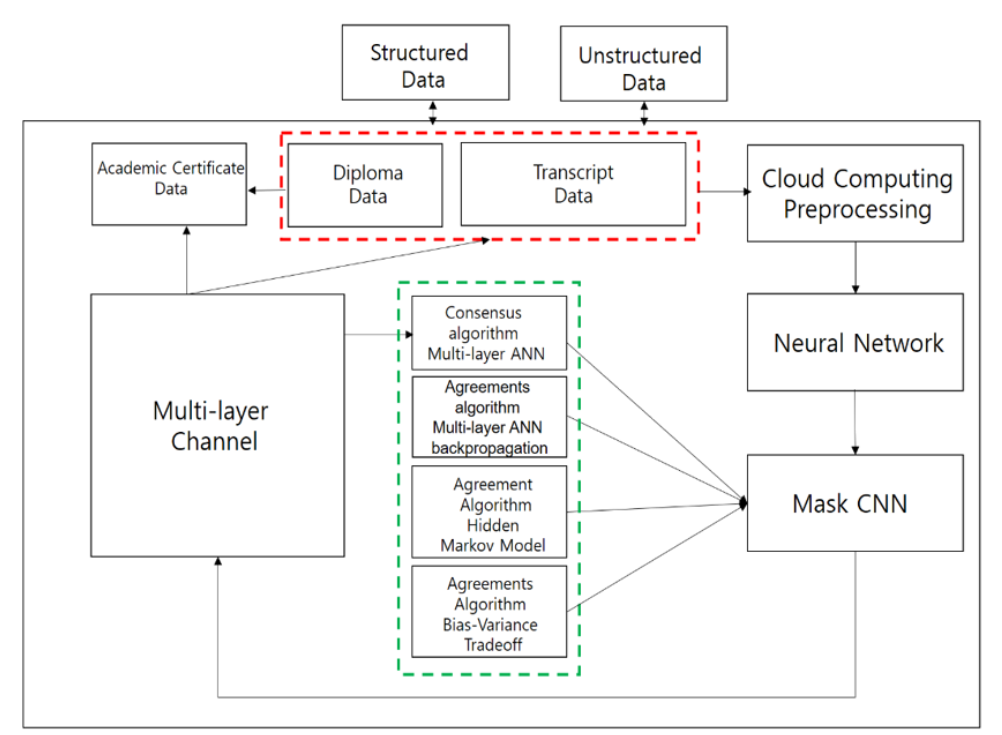
\includegraphics[width=1\linewidth]{images/blockchainforgery.png}
	\end{center}
	\fonte{\cite{blockchainforgery}}
\end{figure}
 
A primeira etapa, "\textit{Cloud Computing Preprocessing}", consiste na entrada e pré-processamento do documento digitalizado e, através de um serviço em nuvem, normaliza os dados brutos da imagem, extrai metadados -- como resolução, dimensões e contraste --, aplica correções de perspectiva e cria uma versão virtualizada semi-persistente do arquivo, preparada para ser processada pelas etapas conseguintes, rejeitando entradas com formato e qualidade inconsistentes.

Em seguida, as imagens passam pela etapa "\textit{Neural Network}", que utiliza \textit{Faster R-CNN} para rapidamente filtrar e detectar artefatos visuais suspeitos. Através de sua rede de propostas regionais (\textit{Region Proposal Network}), o algoritmo captura regiões de interesse -- como selos da universidade, assinaturas, marcas d'água e outros padrões -- e cria escores de confiança para cada uma, identificando áreas possivelmente adulteradas.

Os documentos passam então para a etapa "\textit{Mask CNN}", que através de um modelo \textit{Mask R-CNN} e das regiões de interesse previamente identificadas, segmenta a imagem, criando máscaras binárias a nível de \textit{pixel}, ou seja, para cada região, o algoritmo estima quais \textit{pixels} pertencem ao document legítimo e quais foram forjados. Essas máscaras são então encapsuladas como prova imutável dentro do bloco que será registrado na blockchain, além de servir como outra medida de escore de confiança do documento.

Por fim, ambas as pontuações de confiança são combinadas e passadas ao mecanismo de consenso dessa \textit{blockchain}, representado pela etapa "\textit{Multi-layer Channel}" que, ao invés de utilizar estratégias tradicionais como prova de trabalho ou prova de participação, combina múltiplos algoritmos de aprendizado de máquina. De forma geral, essa arquitetura é composta por quatro componentes principais:

\begin{itemize}
    \item Um algoritmo baseado em uma rede neural multicamadas, que processa os escores de confiança fornecidos pelos processamentos anteriores e, a partir de certo limiar de confidência, imediatamente aprova o documento;
    \item Um algoritmo de aprendizado complementar à rede neural multicamadas, que cruza referências com padrões aprendidos de decisões anteriores -- por exemplo, quando um diploma inicialmente validado como autêntico posteriormente se prova fraudulento -- e ajusta os pesos da rede;
    \item Um algoritmo que utiliza um modelo oculto de Markov para, a partir de uma cadeia de regras, examinar padrões temporais e fornecer avaliações probabilísticas da autenticidade do documento;
    \item Um algoritmo que equilibra a complexidade (\textit{overfitting}) com a generalização (\textit{underfitting}) do modelo de rede neural, ou seja, procura encontrar \textit{trade-off} ótimo entre viés e variância para decisões de consenso confiáveis.
\end{itemize}

Assim, cada nó da \textit{blockchain} executa esses algoritmos e vota, com base na ponderação dos resultados, se devem incluir ou rejeitar o bloco com o diploma. Para qualquer decisão, exige-se quórum de pelo menos $2/3$ de votos. Caso não seja atingido, seja por discordâncias das máscaras ou pela recusa de validadores de alta reputação, uma nova rodada de votação é iniciada com a reexecução das etapas "\textit{Mask CNN}" e "\textit{Multi-layer Channel}" com parâmetros ajustados. Esse ciclo se repete até obter consenso ou direcionar o diploma a uma auditoria humana. Dessa forma, quando um documento é aprovado na rede, é classificado como autêntico no \textit{ledger}; quando reprovado, é sinalizado como fraudulento.

Por fim, quando um terceiro -- como empresa, universidade ou empregador -- deseja verificar a validade de um diploma já registrado, basta a verificação do \textit{hash} do documento já submetido.

\section{``\protect\textit{Multimodal Document Image Classification}``}

O trabalho de \citeauthor*{multimodal} \cite*{multimodal} não lida diretamente com a identificação de documentos falsificados ou fraudados, mas sim do problema geral de classificação de imagens. No entanto, a abordagem utilizada pelos autores é altamente relevante, pois mostra a eficácia da análise multimodal e pode ser aproveitada por este trabalho de conclusão de curso.

O \textit{paper} propõe uma abordagem multimodal para a classificação de imagens de documentos diversos em dezesseis categorias utilizando o \textit{dataset} RVL-CDIP. A proposta combina a fusão de características visuais e textuais para a rotulagem entre imagens e classes. Para isso, segue o \textit{pipeline}:

\begin{enumerate}
    \item Pré-processamento: normaliza e redimensiona as imagens para utilizações posteriores;
    \item Extração de texto: utiliza OCR para extrair texto das páginas;
    \item Extração multimodal, em paralelo:
    \subitem Modalidade textual: utiliza um modelos de linguagem para capturar informações semânticas dos textos extraídos;
    \subitem Modalidade visual: extrai características das imagens a partir de uma rede convolucional;
    \item Fusão multimodal: combina as extrações textuais e visuais;
    \item Classificação final: utiliza uma rede convolucional, que tem como entrada a fusão multimodal, para classificar os documentos.
\end{enumerate}

Para a modalidade textual, os autores trazem à tona o problema de que texto extraído por OCR pode ser muito ruidoso, contendo erros a nível de caracteres ou até palavras. Por isso, capturam representações do conteúdo em três diferentes granularidades. 

A nível de sequência, empregam ULMFiT (\textit{Universal Language Model Fine-tuning}), um modelo que processa o documento como uma sequência de palavras e mantém uma "memória interna", que armazena informações contextuais conforme processa cada palavra sequencialmente. Isso permite que a rede neural capture sequências lógicas, dependências de longo prazo e contexto semântico entre palavras distantes. Como saída, o algoritmo produz uma representação vetorial do texto que leva em consideração as características citadas.

A nível de palavra, para representar cada uma, empregam FastText \textit{embeddings}. A técnica consiste em transformar os termos em vetores numéricos, de forma que palavras com significados similares fiquem próximas no espaço matemático. O vetor final do documento é calculado como a média dos \textit{embeddings} de todas as palavras presentes.

A nível de caractere, para capturar padrões ortográficos, aplicam N-gramas de caracteres -- sequências contínuas de n caracteres abduzidos de uma palavra -- e criam um vetor numérico normalizado das ocorrências dos padrões obtidos.

Em resumo, as características de sequência preservam o contexto semântico geral do documento, as representações de palavra mantêm similaridades semânticas locais, e os N-gramas de caracteres oferecem robustez contra erros de OCR e palavras desconhecidas. Essas três representações são combinadas através de um método \textit{ensemble}, que produz um vetor unificado que comporta essas \textit{features} textuais.

Para a modalidade visual, o trabalho emprega a arquitetura de rede VGG-16 (\textit{Visual Geometry Group}) para extrair características hierárquicas através de suas camadas convolucionais, capturando padrões de layout, tipografia, elementos gráficos e padrões de formatação presentes nos documentos. Como saída, a rede produz um vetor multidimensional que representa uma codificação densa e compacta de todas as informações visuais relevantes do documento.

O principal interesse desse trabalho é a fusão das informações textuais e visuais, que tem por objetivo criar uma representação unificada, que preserve e potencialize as informações complementares de ambas as modalidades, e que permita que um modelo de classificação final explore sinergias entre essas diferentes características. Os autores propõem duas estratégias principais para combinar essas representações, das quais destaca-se a segunda, que combina os vetores anteriormente extraídos.

Essa abordagem explora quatro métodos distintos de junção. De forma geral, o primeiro é a concatenação simples, onde os vetores de características textuais e visuais são diretamente concatenados para formar um vetor unificado. O segundo método utiliza adição elemento a elemento, somando diretamente as representações de ambas as modalidades. O terceiro emprega \textit{compact bilinear pooling}, uma técnica mais sofisticada que calcula o produto externo entre os vetores de características para capturar interações complexas entre as modalidades, permitindo que o modelo de classificação posterior aprenda correlações não-lineares entre informações visuais e textuais. Por fim, o quarto método implementa \textit{multimodal gated units}, que utilizam mecanismos de atenção para aprender uma função de controle que determina automaticamente como ponderar e combinar as características de cada modalidade, o que permite que o modelo posterior adapte dinamicamente a importância relativa de informações visuais ou textuais dependendo do contexto específico do documento -- para documentos altamente textuais como contratos ou relatórios científicos, as características semânticas podem ser mais discriminativas, enquanto para documentos com layouts visuais distintivos como formulários ou apresentações, as características visuais podem ser mais relevantes.

Em sequência, para realizar a classificação final, os autores utilizam uma camada densa e uma camada final \textit{softmax} para a predição, como ilustra a Figura \ref{fig:multimodal}.

\begin{figure}[H]
	\caption{\label{fig:multimodal}Representação da Arquitetura de Fusão Multimodal por \citeauthor*{multimodal}}
    \begin{center}
    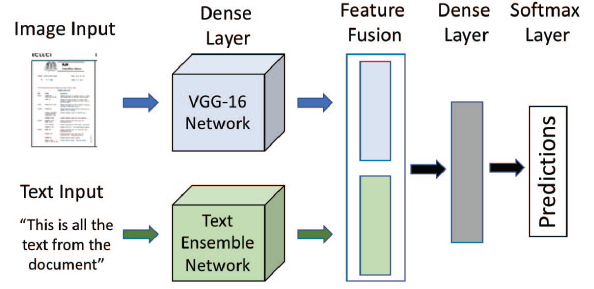
\includegraphics[width=1\linewidth]{images/multimodal.png}
	\end{center}
	\fonte{\cite{multimodal}}
\end{figure}

Finalmente, o artigo compartilha as conclusões finais, onde explicita como essa abordagem superou consistentemente os métodos que utilizam apenas uma modalidade, com o método de adição elemento a elemento curiosamente alcançando os melhores resultados para a fusão multimodal, atingindo uma acurácia de 93,6\% no \textit{dataset} RVL-CDIP.

\section{``\protect\textit{CERTIFICATE FRAUD VERIFICATION MODEL USING CLUSTERED-BASED CLASSIFICATION APPROACH}``}

O trabalho de \citeauthor*{clusterfraudverification} \cite*{clusterfraudverification} lida diretamente com o problema de verificação da autenticidade de certificados acadêmicos. Para isso, propõe uma abordagem baseada em \textit{clustering}, fundamentado na premissa de que documentos legítimos apresentam padrões consistentes de características que podem ser identificados através desses agrupamentos.

O \textit{dataset} utilizado pelos autores consiste em mais de vinte e quatro mil amostras de documentos não rotulados, oficialmente emitidos por duas universidades: Enugu State University of Science and Technology e University of California Irvine.

A metodologia dos autores utiliza o algoritmo K-means como técnica principal para descobrir os padrões dominantes em certificados acadêmicos. Dessa forma, o processo de treinamento consiste na aplicação desse algoritmo sobre as características extraídas dos documentos do \textit{dataset}, com o objetivo de agrupá-los em dezesseis grupos. O algoritmo inicializa centroides e atribui iterativamente cada arquivo ao centroide mais próximo usando um modelo de equidistância. Os centroides são atualizados através do cálculo das médias dos pontos pertencentes a cada \textit{cluster} até atingir convergência. Para a verificação de documentos, o sistema extrai suas características e calcula distâncias em relação aos centroides estabelecidos, classificando-o como legítimo, quando próximo de algum padrão conhecido, ou suspeito, quando distante de todos os \textit{clusters}.

Embora os autores não especifiquem os processos de extração de características, as figuras apresentadas sugerem fortemente o uso de \textit{features} visuais. As imagens, como exemplificado na Figura \ref{fig:clusterfraudverification}, mostram marcações circulares em pontos específicos dos certificados, destacando elementos como logos institucionais e aspectos estruturais dos documentos. Assume-se, portanto, que o sistema captura e converte essas informações em vetores numéricos compatíveis com o K-means.

\begin{figure}[H]
	\caption{\label{fig:clusterfraudverification}Resultado da Verificação de um Documento Autêntico}
    \begin{center}
    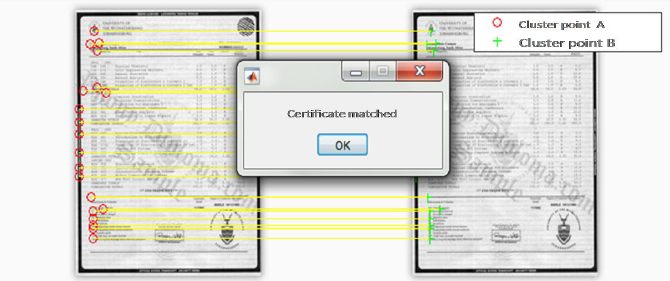
\includegraphics[width=1\linewidth]{images/clusterfraudverification.png}
	\end{center}
	\fonte{\cite{clusterfraudverification}}
\end{figure}

O modelo foi validado experimentalmente com certificados reais e demonstrou capacidade de distinguir documentos autênticos de falsificados, já que os resultados reportaram uma acurácia geral de 86,53\%. Os autores destacam como principal vantagem a capacidade do sistema de operar efetivamente com \textit{datasets} limitados, característica importante em cenários reais onde a disponibilidade de dados rotulados é restrita por questões éticas e de privacidade.